WJW Fox 8
\href{https://web.archive.org/web/20221116194151/https://fox8.com/news/coronavirus/7-ne-ohio-counties-have-some-of-the-highest-coronavirus-spread-in-the-u-s-right-now/}{reports}
that Ashtabula County is one of seven counties in northeast Ohio that is
among the top ten percent in the nation for COVID-19 transmission.
Ashtabula County is specifically ranked as 281st out of 3,142 counties.
That's really, really high.

It isn't as if we're dealing with a low positivity rate on testing or
anything\ldots{}

\begin{figure}
\centering
\pandocbounded{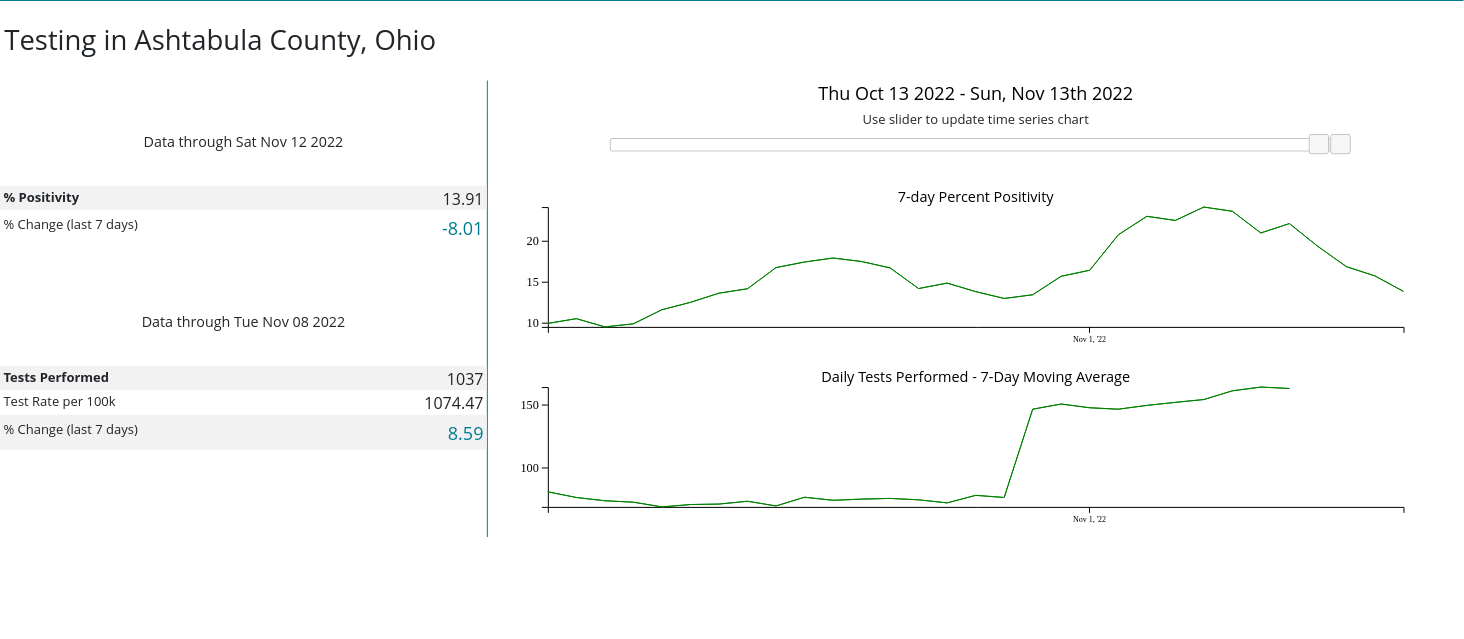
\includegraphics[keepaspectratio]{\%7B\%7Bsite.url\%7D\%7D/img/oct2022-nov2022-covid-testing.png}}
\caption{Export from CDC's reporting portal showing COVID-19 test
positivity from October 13th through November 13th 2022}
\end{figure}

Considering how red this county broke in not just the 2020 General
Election but also the 2022 General Election the inverse correlation of
the presence of COVID denialism is pretty strong. The
\href{https://covid19pvi.niehs.nih.gov/}{Pandemic Vulnerability Index}
is still a sad site to see our county shown on.

This isn't good but there isn't anything I can do to fix the aggregate
problem. I'm as vaccinated as I can be and take all the precautions I
realistically can in this community. Unfortunate outcomes may still be
in the cards for parts of my local community, I fear.
